\documentclass[tikz,border=9pt]{standalone}
\usepackage{fontspec}
\setmainfont{TeX Gyre Heros}
\usepackage{amsmath}
\usepackage{unicode-math}
\setmathfont{TeX Gyre Termes Math}
\usepackage{pgfplots}
\usepgfplotslibrary{fillbetween,groupplots}
\usetikzlibrary{arrows.meta,calc}
\definecolor{maroon}{HTML}{780404}
\definecolor{orange}{HTML}{E37D00}
\definecolor{charcoal}{HTML}{303238}
\definecolor{muted}{HTML}{65686D}
\definecolor{gridgray}{HTML}{DDDFE2}
\pgfplotsset{compat=1.18,
  oscillator/.style={
    width=12.6cm,height=8.8cm,
    xmin=-3.5,xmax=3.5,ymin=0,ymax=5.35,
    axis lines=left,axis line style={charcoal,line width=.7pt,-{Stealth[length=4pt]}},
    xtick={-3,-2,-1,0,1,2,3},ytick={0,1,2,3,4,5},
    tick align=outside,tick style={charcoal},
    tick label style={font=\small,text=charcoal},
    xlabel={$q=x/\ell$},ylabel={$\varepsilon=E/(\hbar\omega)$},
    label style={font=\normalsize,text=charcoal},
    xlabel style={at={(axis description cs:.5,-.085)},anchor=north},
    ylabel style={at={(axis description cs:-.075,.5)},anchor=south},
    ymajorgrids=true,grid style={gridgray,dashed,line width=.35pt},
    clip=false,samples=251,
  },
}
\begin{document}
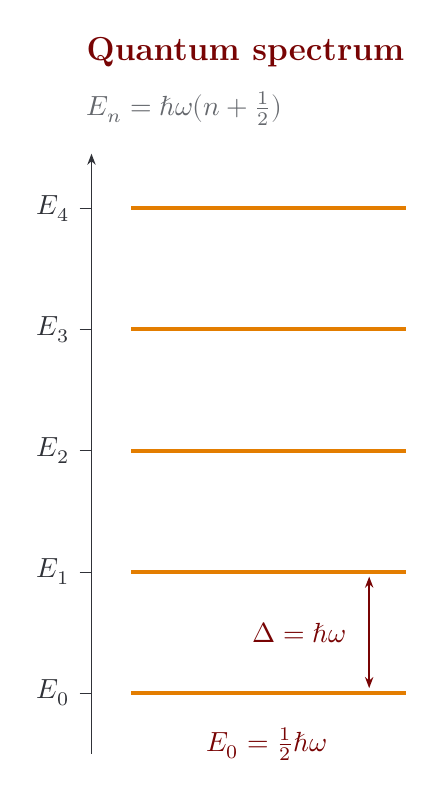
\begin{tikzpicture}[text=charcoal]

\begin{axis}[
  width=6.2cm,height=9.2cm,
  xmin=0,xmax=1.1,ymin=0,ymax=4.95,
  axis x line=none,axis y line=left,
  axis line style={charcoal,line width=.7pt,-{Stealth[length=4pt]}},
  xtick=\empty,ytick={.5,1.5,2.5,3.5,4.5},
  yticklabels={$E_0$,$E_1$,$E_2$,$E_3$,$E_4$},
  tick align=outside,tick style={charcoal},
  tick label style={font=\normalsize,text=charcoal},
  ylabel={},
  clip=false,
]
\node[anchor=west,font=\large\bfseries,text=maroon]
  at (axis description cs:-.04,1.17) {Quantum spectrum};
\node[anchor=west,font=\normalsize,text=muted]
  at (axis description cs:-.04,1.075) {$E_n=\hbar\omega(n+\tfrac12)$};
\foreach \level in {.5,1.5,2.5,3.5,4.5}{
  \addplot[orange,line width=1.5pt] coordinates {(.12,\level) (.95,\level)};
}
\draw[maroon,line width=.9pt,{Stealth[length=4pt]}-{Stealth[length=4pt]}]
  (axis cs:.84,.54)--(axis cs:.84,1.46);
\node[anchor=east,text=maroon,font=\normalsize,xshift=-5pt]
  at (axis cs:.84,1) {$\Delta=\hbar\omega$};
\node[anchor=north,text=maroon,font=\normalsize,yshift=-9pt]
  at (axis cs:.53,.5) {$E_0=\tfrac12\hbar\omega$};
\end{axis}
\end{tikzpicture}
\end{document}
